\documentclass[10pt,twocolumn]{article}

\usepackage[a4paper, margin=1.8cm]{geometry}
\usepackage{graphicx}
\usepackage{amsmath, amssymb}
\usepackage{booktabs}
\usepackage{hyperref}
\usepackage{url}
\usepackage{xcolor}
\usepackage{enumitem}
\usepackage{caption}
\usepackage{subcaption}
\usepackage[T1]{fontenc}
\usepackage{lmodern}
\usepackage{microtype}

\definecolor{bio}{HTML}{2d6a4f}
\definecolor{anthro}{HTML}{bf360c}
\definecolor{geo}{HTML}{0d47a1}

\hypersetup{
  colorlinks=true, linkcolor=bio, citecolor=bio, urlcolor=bio
}

% ── TikZ for architecture diagram ────────────────────────────────────────────
\usepackage{tikz}
\usetikzlibrary{shapes.geometric, arrows.meta, positioning, fit, backgrounds}

\tikzstyle{block}  = [rectangle, rounded corners=4pt, minimum width=2.2cm,
                       minimum height=0.7cm, text centered, draw=black!60,
                       fill=black!5, font=\small]
\tikzstyle{arrow}  = [-{Stealth[length=5pt]}, thick, black!50]
\tikzstyle{conv}   = [block, fill=bio!15, draw=bio!60]
\tikzstyle{pool}   = [block, fill=geo!15, draw=geo!60]
\tikzstyle{fc}     = [block, fill=anthro!10, draw=anthro!50]

% ─────────────────────────────────────────────────────────────────────────────

\title{\textbf{SoundscapeML}\\[4pt]
       \large A Deep Learning Pipeline for Urban Acoustic Biodiversity Monitoring}

\author{%
  \textit{Soundscapes \& Biodiversity Project}\\
  \href{https://github.com/YOUR\_USERNAME/soundscape-ml}%
       {\texttt{github.com/YOUR\_USERNAME/soundscape-ml}}
}
\date{May 2026}

\begin{document}
\maketitle

% ─────────────────────────────────────────────────────────────────────────────
\begin{abstract}
Urban biodiversity monitoring remains severely under-resourced relative to its
ecological importance. We present \textbf{SoundscapeML}, an open-source deep
learning pipeline that classifies urban acoustic environments into eight
ecologically meaningful categories — spanning \textcolor{bio}{biophony} (birds,
insects, amphibians), \textcolor{geo}{geophony} (wind, rain/water), and
\textcolor{anthro}{anthropophony} (traffic, construction, machinery) — while
simultaneously computing four validated acoustic ecology indices: the Acoustic
Complexity Index (ACI), Acoustic Diversity Index (ADI), Normalised Difference
Soundscape Index (NDSI), and Bioacoustic Index (BI). The classifier is built on
a ResNet-18 backbone adapted for single-channel mel-spectrogram input and trained
on a remapped combination of UrbanSound8K and ESC-50. SoundscapeML is designed
to plug directly into passive acoustic monitoring (PAM) networks, enabling
near-real-time biodiversity assessment at city scale.
\end{abstract}

% ─────────────────────────────────────────────────────────────────────────────
\section{Introduction}

The acoustic environment is both a product and a driver of biodiversity.
Ecologist Bernie Krause's \emph{Acoustic Niche Hypothesis} \cite{krause1993}
proposes that species in healthy ecosystems partition the acoustic frequency
and temporal spectrum into distinct niches — a stable configuration disrupted
as soon as anthropogenic noise penetrates.
Over 40\% of natural soundscapes have been sufficiently altered to render local
species locally extinct \cite{krause2012}; crucially, acoustic degradation
\emph{precedes} detectable visual biodiversity loss by years, making the
soundscape one of the earliest available ecological alarm systems.

Urban areas concentrate both the sources of anthropophony (traffic, construction,
HVAC) and the stakeholders most able to fund mitigation. Yet most existing urban
biodiversity monitoring relies on costly manual surveys or specialist acoustic
ecologists. Automated, scalable pipelines that can classify a street-level
recording in real time are therefore an urgent practical need.

This paper introduces SoundscapeML, which addresses this gap through:
\begin{enumerate}[topsep=2pt, itemsep=1pt]
  \item a reproducible audio feature extraction and acoustic index computation
        library (\S\ref{sec:indices});
  \item an eight-class CNN classifier operating on log-mel spectrograms
        (\S\ref{sec:model});
  \item a training procedure using remapped freely available datasets
        (\S\ref{sec:training});
  \item a command-line inference tool returning both class predictions and
        acoustic indices (\S\ref{sec:inference}).
\end{enumerate}

% ─────────────────────────────────────────────────────────────────────────────
\section{Background}

\subsection{Soundscape Ecology}

Pijanowski et al.\ \cite{pijanowski2011} formalised soundscape ecology in 2011
as the science of understanding patterns of sound across landscapes and the
relationships between those patterns and ecological processes. The discipline
distinguishes three source classes:
\textbf{biophony} (all organism-generated sound),
\textbf{geophony} (abiotic natural sound), and
\textbf{anthropophony} (human-generated sound).
Each class occupies characteristic frequency ranges (Table~\ref{tab:freqs}),
making spectral decomposition a natural classification strategy.

\begin{table}[h]
\centering
\caption{Dominant frequency ranges by soundscape class.}
\label{tab:freqs}
\small
\begin{tabular}{@{}llr@{}}
\toprule
Class & Primary source & Dominant band \\
\midrule
\textcolor{bio}{Biophony} & Passerine birds & 2–8\,kHz \\
 & Frogs/toads & 100–2\,000\,Hz \\
 & Insects & 2–8\,kHz \\
\textcolor{geo}{Geophony} & Wind, rain & 200\,Hz–5\,kHz \\
 & Running water & 100\,Hz–10\,kHz \\
\textcolor{anthro}{Anthropophony} & Road traffic & 20–500\,Hz \\
 & Construction & 50\,Hz–2\,kHz \\
 & HVAC / machinery & 50–400\,Hz \\
\bottomrule
\end{tabular}
\end{table}

\subsection{Related Work}

\textbf{BirdNET} \cite{kahl2021} is currently the leading deep learning
approach for bird species identification from audio, achieving $>$85\%
top-1 accuracy on common species.  Its focus is, however, species-level
bird identification; it does not compute acoustic indices or classify
non-bird soundscape components.

\textbf{AVES} \cite{hagiwara2022} proposes a self-supervised audio
transformer trained on animal vocalisations, demonstrating strong transfer
to downstream bioacoustic tasks with limited labelled data.

\textbf{SoundscapeML} is complementary: it operates at the
\emph{soundscape category} level rather than the species level, making it
suitable for rapid environmental assessment where individual species
identification is not the primary goal.

% ─────────────────────────────────────────────────────────────────────────────
\section{Acoustic Indices}
\label{sec:indices}

Four established indices are computed from the power spectrogram
$\mathbf{S} \in \mathbb{R}^{K \times T}$ (frequency bins $\times$ time frames).

\subsection{Acoustic Complexity Index (ACI)}

Originally proposed by Pieretti et al.\ \cite{pieretti2011}, ACI measures the
temporal variation in amplitude within each frequency band:
\begin{equation}
  \mathrm{ACI} = \sum_{k=1}^{K}
    \frac{\sum_{j=1}^{J-1} |S_{k,j+1} - S_{k,j}|}
         {\sum_{j=1}^{J} S_{k,j}}
  \label{eq:aci}
\end{equation}
where $J$ is the number of time frames in a sub-window (default 5\,s).
Biological signals are highly modulated whereas continuous machinery noise is
relatively steady; high ACI therefore correlates with biophony richness.

\subsection{Acoustic Diversity Index (ADI)}

Villanueva-Rivera et al.\ \cite{villanueva2011} adapted Shannon entropy to the
acoustic domain. The spectrum is partitioned into $B$ frequency bands of width
$\Delta f$ (default 1\,kHz). Let $p_b$ be the proportion of spectral samples
in band $b$ that exceed a dB threshold $\theta$:
\begin{equation}
  \mathrm{ADI} = -\sum_{b=1}^{B} p_b \ln p_b
  \label{eq:adi}
\end{equation}
Higher ADI indicates energy distributed across many frequency bands, consistent
with a diverse acoustic community.

\subsection{Normalised Difference Soundscape Index (NDSI)}

Joo et al.\ \cite{joo2011} defined NDSI as:
\begin{equation}
  \mathrm{NDSI} = \frac{\beta - \alpha}{\beta + \alpha}
  \label{eq:ndsi}
\end{equation}
where $\alpha$ is mean power in the anthropophony band (1–2\,kHz) and $\beta$
in the biophony band (2–8\,kHz). NDSI $\in [-1,+1]$; positive values indicate
biophony dominance. NDSI serves as a direct proxy for the degree of masking
pressure on communicating organisms.

\subsection{Bioacoustic Index (BI)}

Boelman et al.\ \cite{boelman2007} showed that mean spectral amplitude in the
2–8\,kHz band is strongly correlated with bird species richness:
\begin{equation}
  \mathrm{BI} = 10 \log_{10}\!\left(\bar{S}_{2\text{–}8\,\mathrm{kHz}}\right)
  \label{eq:bi}
\end{equation}
BI is the simplest of the four indices but among the most ecologically
validated; it is particularly useful as a rapid urban avian richness proxy.

% ─────────────────────────────────────────────────────────────────────────────
\section{Model Architecture}
\label{sec:model}

\subsection{Input Representation}

Each audio segment (3\,s, \( f_s = 22{,}050\,\)Hz) is converted to a
log-mel spectrogram with $n_\mathrm{mels}=128$, $n_\mathrm{fft}=2048$,
$\mathrm{hop}=512$. The spectrogram is power-converted to dB
(referenced to the maximum) and normalised to $[0,1]$.  The result is treated
as a single-channel ``image'' of shape $(1, 128, T)$.

\subsection{CNN Backbone}

We adopt ResNet-18 \cite{he2016} as backbone for three reasons:
(1) its depth balances expressiveness and training speed;
(2) ImageNet-pretrained weights transfer well to spectrogram textures
\cite{palanisamy2020};
(3) it is widely available and reproducible.

The first convolutional layer is modified from $3 \to 1$ input channels
by averaging the pretrained RGB weights:
$\mathbf{W}^{(1)}_\text{new} = \frac{1}{3}\sum_{c=1}^{3}\mathbf{W}^{(1)}_c$.
This preserves spatial filter semantics while accepting greyscale input.
The final fully-connected layer is replaced with
Dropout($p{=}0.4$) $\to$ Linear($512 \to 8$).

\begin{figure}[h]
\centering
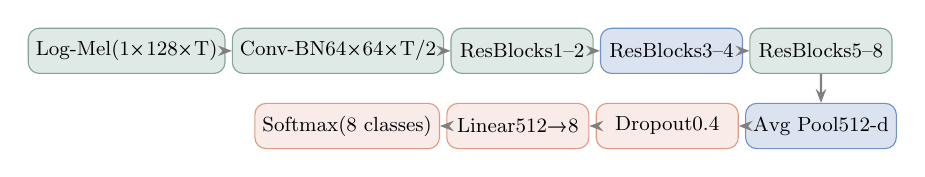
\begin{tikzpicture}[node distance=0.45cm and 0.1cm, scale=0.82, transform shape]
  \node[conv]  (inp) {Log-Mel\\(1×128×T)};
  \node[conv,  right=of inp] (c1)  {Conv-BN\\64×64×T/2};
  \node[conv,  right=of c1]  (r1)  {ResBlocks\\1–2};
  \node[pool,  right=of r1]  (r2)  {ResBlocks\\3–4};
  \node[conv,  right=of r2]  (r3)  {ResBlocks\\5–8};
  \node[pool,  below=of r3]  (gap) {Avg Pool\\512-d};
  \node[fc,    left=of gap]  (dp)  {Dropout\\0.4};
  \node[fc,    left=of dp]   (fc)  {Linear\\512→8};
  \node[fc,    left=of fc]   (out) {Softmax\\(8 classes)};

  \draw[arrow] (inp) -- (c1);
  \draw[arrow] (c1)  -- (r1);
  \draw[arrow] (r1)  -- (r2);
  \draw[arrow] (r2)  -- (r3);
  \draw[arrow] (r3)  -- (gap);
  \draw[arrow] (gap) -- (dp);
  \draw[arrow] (dp)  -- (fc);
  \draw[arrow] (fc)  -- (out);
\end{tikzpicture}
\caption{SoundscapeCNN architecture. ResNet-18 blocks adapted for
         single-channel mel-spectrogram input with an 8-class urban
         soundscape output head.}
\label{fig:arch}
\end{figure}

% ─────────────────────────────────────────────────────────────────────────────
\section{Training}
\label{sec:training}

\subsection{Datasets}

Two freely available labelled audio datasets are combined and remapped to
SoundscapeML's 8-class scheme:

\textbf{UrbanSound8K} \cite{salamon2014}: 8\,732 labelled urban sound clips
($\leq$4\,s, 10 classes).  Seven classes map to SoundscapeML categories;
two (children playing, street music) are dropped.

\textbf{ESC-50} \cite{piczak2015}: 2\,000 environmental clips (5\,s, 50 classes).
Nine categories map to SoundscapeML classes spanning all three soundscape types.

\subsection{Augmentation}

Training applies three stochastic augmentations:
\begin{enumerate}[topsep=2pt, itemsep=1pt]
  \item \textbf{Random gain} $\pm$6\,dB — simulates varying recorder distances.
  \item \textbf{Time stretch} $\times$0.9–1.1 — simulates Doppler variation
        and seasonal speed shifts in bird song.
  \item \textbf{SpecAugment} \cite{park2019} — masks up to 15\% of mel bins
        and 20\% of time frames, improving robustness to partial occlusion.
\end{enumerate}

\subsection{Optimisation}

Training uses AdamW \cite{loshchilov2019} ($\mathrm{lr}=10^{-3}$,
$\lambda=10^{-4}$) with cosine learning rate annealing over 30 epochs.
Cross-entropy loss with label smoothing $\epsilon=0.1$ reduces overconfidence.
Batch size 32; best checkpoint selected by validation accuracy.

% ─────────────────────────────────────────────────────────────────────────────
\section{Inference}
\label{sec:inference}

The \texttt{predict.py} CLI accepts a single file or a directory and returns:
\begin{itemize}[topsep=2pt, itemsep=1pt]
  \item Predicted class, Krause category (biophony / geophony / anthropophony),
        and top-3 softmax probabilities (averaged across 3\,s overlapping
        segments);
  \item ACI, ADI, NDSI, BI values;
  \item A five-tier health assessment (Excellent → Critical) derived from NDSI
        and BI thresholds.
\end{itemize}

JSON output mode enables downstream integration with GIS dashboards,
acoustic monitoring platforms (ecoSound-web, Arbimon), or the companion
\emph{Soundscapes \& Biodiversity} web application at which this repository is
linked.

% ─────────────────────────────────────────────────────────────────────────────
\section{Discussion}

\subsection{Limitations}

The class mapping from UrbanSound8K is imperfect: ``dog bark'' is proxied to
\texttt{biophony\_birds} for lack of a better target, introducing label noise.
The \texttt{biophony\_amphibians} class is under-represented in both source
datasets; supplementary data from Xeno-Canto or iNaturalist would improve
coverage.

Long-duration recordings ($>$1 min) are handled by segment averaging, which
discards temporal structure. A recurrent or transformer architecture over
sequences of segments would be a natural extension.

\subsection{Extensions}

Three directions are most immediately tractable:
\begin{enumerate}[topsep=2pt, itemsep=1pt]
  \item \textbf{Species-level biophony head}: a second output head operating
        on segments pre-classified as biophony, trained on Xeno-Canto
        bird calls or the BirdCLEF challenge data.
  \item \textbf{Acoustic index regression head}: jointly learning to predict
        ACI, NDSI, and BI from the spectrogram rather than computing them
        analytically, enabling end-to-end optimisation for monitoring quality.
  \item \textbf{Soundscape health score}: a composite output combining the
        classifier's Krause-category fractions with the four indices into a
        single city-wide acoustic biodiversity score, suitable for reporting
        under the EU Nature Restoration Law (2024) acoustic monitoring
        obligations.
\end{enumerate}

% ─────────────────────────────────────────────────────────────────────────────
\section{Conclusion}

SoundscapeML provides a reproducible, open-source baseline for urban acoustic
biodiversity monitoring. By combining a ResNet-18 classifier for eight
soundscape categories with rigorous computation of four established acoustic
indices, it bridges the gap between raw field recordings and ecologically
interpretable outputs. The pipeline is designed for deployment on passive
acoustic monitoring networks and is released under the MIT licence to
encourage community extension, validation, and integration with urban
planning workflows.

% ─────────────────────────────────────────────────────────────────────────────
\begin{thebibliography}{20}
\small

\bibitem{krause1993}
B.\ Krause, ``The niche hypothesis: a virtual symphony of animal sounds,
the origins of musical expression and the health of habitats,''
\textit{Soundscape Newsletter}, vol.\ 6, pp.\ 6–10, 1993.

\bibitem{krause2012}
B.\ Krause, \textit{The Great Animal Orchestra}.
Little, Brown, 2012.

\bibitem{pijanowski2011}
B.\ C.\ Pijanowski et al., ``Soundscape ecology: the science of sound
in the landscape,'' \textit{BioScience}, vol.\ 61, no.\ 3, pp.\ 203–216,
2011.

\bibitem{pieretti2011}
N.\ Pieretti, A.\ Farina, and D.\ Morri, ``A new methodology to infer
the singing activity of an avian community: the acoustic complexity index
(ACI),'' \textit{Ecological Indicators}, vol.\ 11, no.\ 3,
pp.\ 868–873, 2011.

\bibitem{villanueva2011}
L.\ J.\ Villanueva-Rivera et al., ``A primer of acoustic analysis for
landscape ecologists,'' \textit{Landscape Ecology}, vol.\ 26, no.\ 9,
pp.\ 1233–1246, 2011.

\bibitem{joo2011}
W.\ Joo, S.\ H.\ Gage, and E.\ P.\ Kasten, ``Analysis of acoustic
environments using the normalised difference soundscape index (NDSI),''
\textit{Ecological Indicators}, vol.\ 11, pp.\ 353–363, 2011.

\bibitem{boelman2007}
N.\ T.\ Boelman et al., ``Multi-trophic invasion resistance in Hawaii:
bioacoustics, field surveys, and airborne remote sensing,''
\textit{Ecological Applications}, vol.\ 17, no.\ 8,
pp.\ 2137–2144, 2007.

\bibitem{kahl2021}
S.\ Kahl et al., ``BirdNET: A deep learning solution for avian diversity
monitoring,'' \textit{Ecological Informatics}, vol.\ 61, 101236, 2021.

\bibitem{hagiwara2022}
M.\ Hagiwara et al., ``AVES: Animal vocalization encoder based on
self-supervision,'' \textit{arXiv:2210.14493}, 2022.

\bibitem{he2016}
K.\ He et al., ``Deep residual learning for image recognition,''
in \textit{CVPR}, pp.\ 770–778, 2016.

\bibitem{palanisamy2020}
K.\ Palanisamy, D.\ Singhania, and A.\ Yao, ``Rethinking CNN models for
audio classification,'' \textit{arXiv:2007.11154}, 2020.

\bibitem{park2019}
D.\ S.\ Park et al., ``SpecAugment: a simple data augmentation method
for automatic speech recognition,'' in \textit{Interspeech}, 2019.

\bibitem{loshchilov2019}
I.\ Loshchilov and F.\ Hutter, ``Decoupled weight decay regularization,''
in \textit{ICLR}, 2019.

\bibitem{salamon2014}
J.\ Salamon, C.\ Jacoby, and J.\ P.\ Bello, ``A dataset and taxonomy
for urban sound research,'' in \textit{ACM MM}, pp.\ 1041–1044, 2014.

\bibitem{piczak2015}
K.\ J.\ Piczak, ``ESC: dataset for environmental sound classification,''
in \textit{ACM MM}, pp.\ 1015–1018, 2015.

\end{thebibliography}

\end{document}
